    \subsection{Performance Analysis}
    \label{subsec:performance-analysis}

    This subsection presents the experimental evaluation of VeRedact-PQ
    under increasing redaction workloads, committee configurations, audit
    scopes, and on-chain anchoring costs. The objective is to assess whether
    the proposed batching, coalescing, and cost-aware auditing mechanisms
    improve end-to-end redaction efficiency while preserving the
    request-level validation and post-quantum protection defined in
    Section~\ref{sec:security}.

    \subsubsection{Experimental Setup}

    \chg{VeRedact-PQ, the four redactable-blockchain
    baselines~\cite{ref1,ref13,ref27,ref34}, and the post-quantum batch
    authentication scheme of~\cite{ref39} were
    implemented in approximately 9{,}900 lines of Python, Rust, and Solidity
    code and evaluated on an AWS \chg{r7i.4xlarge} server with an Intel Xeon
    Platinum 8488C processor (16 vCPUs) and \chg{128}\,GB RAM, running Ubuntu 24.04.
    The Besu validator nodes ran as Docker containers on this host, and
    inter-node latency was set to 10\,ms using Linux \texttt{tc netem} to
    emulate a multi-organization deployment; committee members, the VPS, the
    audit service, and the auditor ran as processes on the same host. In
    Experiment~1, requesters generated their signatures and PQZK proofs on
    two separate c7i.48xlarge hosts, so that requester-side proving did not
    consume the cores of the system under test.}

    PQSIG was instantiated with ML-DSA-65 (FIPS~204) through the Open Quantum
    Safe \texttt{liboqs} library. $H$, $H_1$, $H_2$, and $H_A$ were
    instantiated as domain-separated SHA3-256, and $\mathsf{PRF}$ as
    HMAC-SHA3-256 with 256-bit keys $K_{\mathrm{idx}}$
    and $K_A$ { ($\lambda=256$)}, consistent with the {$\lambda$}-bit key length of Phase~1. PQZK was instantiated with a transparent hash-based
    STARK proof system \chg{(winterfell~0.13; 42 queries, blowup factor~8,
    16-bit grinding)}, consistent with the
    trapdoor-free setup assumed in Phase~1. PQCH was implemented as an
    SIS-based chameleon hash following~\cite{ref10,ref17}, with distributed
    adaptation realized through $t$-of-$n$ trapdoor sharing
    \chg{of a gadget-based lattice trapdoor, dealt without a trusted dealer}. Merkle structures, BIMC, SA-RLI,
    and RAI use binary SHA3-256 trees with multiproof support. The PBN was
    deployed as a \chg{7}-validator Hyperledger Besu network using
    QBFT consensus \chg{with a 2-s block period}, with Solidity contracts anchoring policy commitments,
    committee configurations, batch checkpoints, and RAI checkpoints; PQ
    signature verification is performed by the validator nodes before
    anchoring rather than inside the contracts. Table~\ref{tab:primitives}
    reports the measured execution time of each primitive.

    The workload consists of synthetic enterprise transactions with payloads
    of 256\,B to 4\,KB, organized into transaction batches of $N$ leaves.
    Redaction targets follow a Zipf distribution with skew $s$ to control
    batch locality, where $s=0$ corresponds to uniformly distributed targets
    and larger $s$ concentrates requests on fewer transaction batches.
    Request arrivals follow a Poisson process whose rate is varied per
    experiment\chg{, and every scheme replays the same request trace generated
    from one seed}.
    Unless otherwise stated, the parameters in Table~\ref{tab:params} are
    used\chg{. Each configuration point is executed once; reported values are
    medians (95th percentiles for latency) over all requests or samples of
    that run, and primitive timings are medians with 95\% confidence
    intervals.}

    To separate architectural effects from primitive choice, all baselines were reimplemented within the same framework and
    instantiated with their own classical primitives at about 128-bit
    security, since none of their papers defines a post-quantum variant.
    \chg{As a post-quantum reference point, Scheme~\cite{ref39} (LETA) is
    also included: it authenticates a batch of requests with module-lattice
    signatures and a per-requester zero-knowledge proof, which a leader
    aggregates and a single verifier checks. It was instantiated on the
    ML-DSA ring ($n=256$, $q=8{,}380{,}417$) with module rank~5, the security
    level of VeRedact-PQ. Since it defines no redaction, audit, or on-chain
    step, it enters only Table~\ref{tab:primitives} and Experiment~2.}
    Stages not
    defined by a baseline's paper are reported as not supported. Each baseline otherwise follows its original
    workflow, including per-request authorization and adaptation.
    \chg{For auditing, Scheme~\cite{ref1} holds its accumulator membership
    proofs locally, an option its paper provides, and the per-record
    accumulator witnesses of Scheme~\cite{ref13} are timed individually on one
    core and summed. The redaction histories audited in Experiments~3 and~4
    are built beforehand and are not timed. Since the paper of
    Scheme~\cite{ref1} fixes no block size and its chain permits one
    redaction per block, each of its blocks holds one transaction, so that
    its history reaches the largest audit point.}

    \begin{table}[t]
    \centering
    \caption{Execution Time of Cryptographic Primitives}
    \label{tab:primitives}
    \scriptsize
    \renewcommand{\arraystretch}{1.08}
    \setlength{\tabcolsep}{4pt}
    \begin{tabular}{llc}
    \hline
    \textbf{Operation} & \textbf{Instantiation} & \textbf{Time (ms)} \\
    \hline
    \multicolumn{3}{l}{\textit{VeRedact-PQ}} \\
    $T_S$ / $T_V$ & ML-DSA-65 sign / verify & \chg{0.085 / 0.032} \\
    $T_{ZP}$ / $T_{ZV}$ & PQZK prove / verify & \chg{22.898 / 0.722} \\
    $T_{CH}$ & PQCH hash & \chg{1.196} \\
    $T_{PA}$ / $T_{CB}$ & PQCH partial adapt / combine & \chg{18.835 / 5.820} \\
    $T_H$ & SHA3-256 (64-byte input) & \chg{0.001} \\
    $T_{\mathrm{PRF}}$ & HMAC-SHA3-256 & \chg{0.004} \\
    \hline
    \multicolumn{3}{l}{\textit{Baselines}} \\
    $T_V^{c}$ & ECDSA secp256k1 verify~\cite{ref1,ref27} & \chg{0.028 / 0.027} \\
    $T_{PA}^{c}$ / $T_{CV}^{c}$ & Improved DCH, BLS12-381~\cite{ref1} & \chg{0.666 / 2.838} \\
    $T_{PA}^{c}$ / $T_{CV}^{c}$ & ETCH, secp256k1~\cite{ref27} & \chg{0.038 / 0.057} \\
    $T_{AD}^{c}$ / $T_{CV}^{c}$ & Double-trapdoor CH, RSA-3072~\cite{ref13} & \chg{7.989 / 8.516} \\
    $T_{AD}^{c}$ / $T_{CV}^{c}$ & CHET, RSA-3072~\cite{ref34} & \chg{56.813 / 50.662} \\
    $T_{Acc}$ & RSA-3072 accumulator~\cite{ref1,ref13} & \chg{0.760} \\
    $T_{Tag}$ & Identity-based RSA-3072 tag~\cite{ref13} & \chg{62.187 / 54.689} \\
    $T_{Pol}$ & MA-ABE decryption, BLS12-381~\cite{ref34} & \chg{7.716} \\
    \chg{$T_E^{c}$} & \chg{RSA-3072 exponentiation~\cite{ref13}} & \chg{7.761} \\
    \hline
    \multicolumn{3}{l}{\chg{\textit{Post-quantum baseline}}} \\
    \chg{$T_m^{L}$} & \chg{Polynomial multiplication in $R_q$~\cite{ref39}} & \chg{0.265} \\
    \chg{$T_S^{L}$ / $T_{ZV}^{L}$} & \chg{Lattice sign + ZKP / ZKP verify~\cite{ref39}} & \chg{1.031 / 0.725} \\
    \chg{$T_{AG}^{L}$ / $T_{AV}^{L}$} & \chg{Aggregate / verify, 64 signatures~\cite{ref39}} & \chg{13.745 / 20.169} \\
    \hline
    \end{tabular}
    \end{table}

    \begin{table}[t]
    \centering
    \caption{Default Experimental Parameters}
    \label{tab:params}
    \scriptsize
    \renewcommand{\arraystretch}{1.08}
    \setlength{\tabcolsep}{4pt}
    \begin{tabular}{ll}
    \hline
    \textbf{Parameter} & \textbf{Default value} \\
    \hline
    Committee size $n$ / threshold $t$ & [7] / [5] \\
    ABRRR bounds $B_{\min}$ / $B_{\max}$ & [8] / [256] \\
    Maximum waiting time $T_{\max}$ & [500]\,ms \\
    Transaction leaves per batch $N$ & [256] \\
    SA-RLI shards $S$ / RAI shards $S_A$ & [16] / [16] \\
    Ledger size & \chg{[$10^6$]} transactions \\
    Zipf skew $s$ & [0.8] \\
    Signature scheme & ML-DSA-65 (NIST category 3) \\
    \chg{Runs} & \chg{1 per point; 30 samples per point (Exp.~2--4), 5 at $n_Q=10^5$} \\
    \hline
    \end{tabular}
    \end{table}

    % ---------------------------------------------------------------------
    \subsubsection*{\textbf{Experiment 1: Redaction Latency and Throughput}}

    This experiment evaluates end-to-end redaction performance \chg{as the
    request arrival rate increases from 1 to 1{,}000 requests/s, the same
    rates for every scheme} over the
    default ledger, \chg{comparing VeRedact-PQ with Refs.~\cite{ref1},
    \cite{ref13}, \cite{ref27}, and~\cite{ref34}}. End-to-end latency is
    measured from request \chg{arrival} to blockchain finalization of the
    updated checkpoint, covering Phases~3 to~5\chg{, over every request that
    arrives in the measurement window; a request not finalized by the end of
    a 30-s drain period is counted with its elapsed time at that moment, and
    latency is reported only at rates where at least 95\% of these requests
    are finalized, so that every reported value is a complete measurement},
    and throughput is measured as
    \chg{the number of redactions finalized per second within a 60-s window
    that follows a 10-s warm-up}. The results are shown in
    Fig.~\ref{fig:exp1_redaction}.

    \begin{figure}[t]
    \centering
    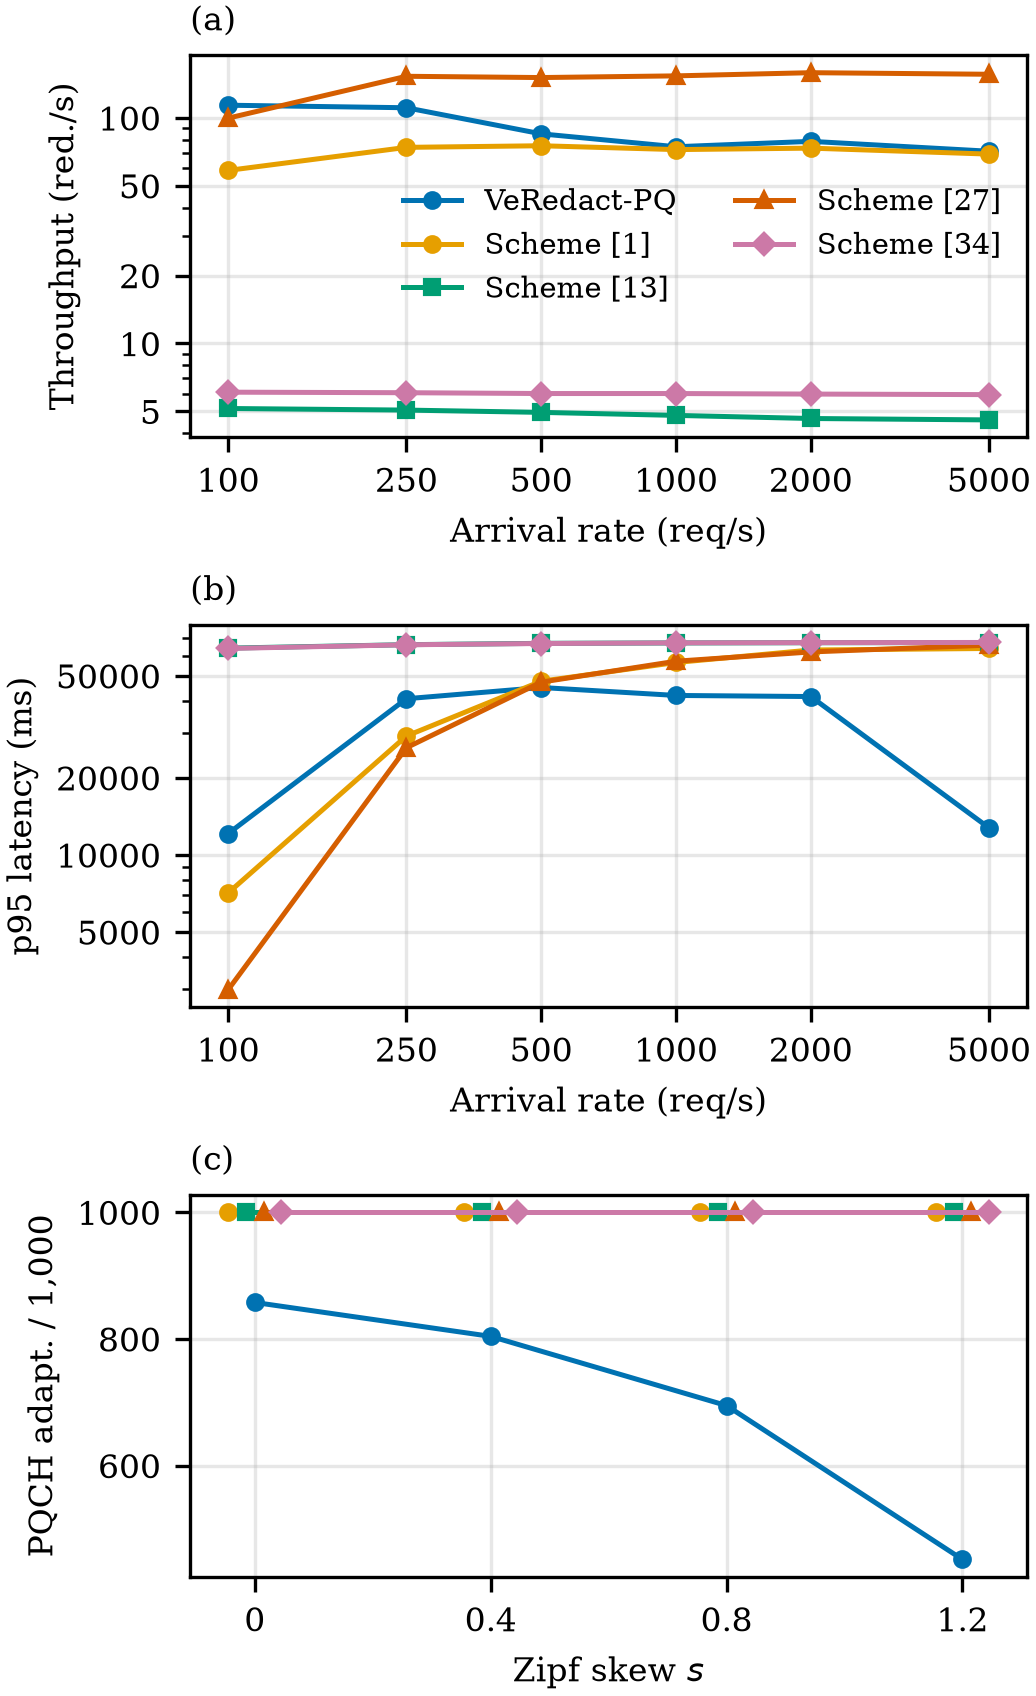
\includegraphics[width=0.8\linewidth]{exp1_redaction_throughput.png}
    \caption{Redaction performance: (a) throughput and
    (b) 95th-percentile end-to-end latency versus request arrival rate.}
    \label{fig:exp1_redaction}
    \end{figure}

    % TODO 2026-10-23: the two results paragraphs below are from the 10^6 run at 100-5,000 req/s;
    % rewrite them after the Exp. 1 rerun of every scheme at 1-1,000 req/s.
    \chg{Fig.~\ref{fig:exp1_redaction}(a) shows that Ref.~\cite{ref27}
    achieves the highest throughput, about 128--145 redactions/s from
    250 requests/s onward, consistent with its low-cost classical adaptation
    ($T_{PA}^{c}=0.038$\,ms per redactor in Table~\ref{tab:primitives}).
    VeRedact-PQ finalizes 99 and 138 redactions/s at 100 and 250
    requests/s and 65--109 redactions/s at higher rates, whereas each of its
    distributed PQCH adaptations requires post-quantum partial adaptations
    ($T_{PA}=18.8$\,ms per member). Ref.~\cite{ref1} reaches 65--72
    redactions/s; its chain additionally permits only one redaction per block,
    so requests to an already redacted block are rejected. Refs.~\cite{ref13}
    and~\cite{ref34} saturate at about 5 and 6 redactions/s, consistent with
    the RSA-3072 tag and CHET operations of about 57--62\,ms each that every
    redaction requires.}

    \chg{Fig.~\ref{fig:exp1_redaction}(b) reports the 95th-percentile
    end-to-end latency on a logarithmic scale. At 100 requests/s, every
    request of VeRedact-PQ and Ref.~\cite{ref27} is finalized, with 3.2
    and 3.4\,s, respectively, and Ref.~\cite{ref1} requires 31.0\,s, whereas
    Refs.~\cite{ref13} and~\cite{ref34} finalize none of the requests
    arriving in the window before the drain ends, so their latency is at
    least 87\,s at every rate. At 250 requests/s, VeRedact-PQ,
    Ref.~\cite{ref27}, and Ref.~\cite{ref1} exceed their throughput and
    leave 29\%, 40\%, and 70\% of the requests unfinished, giving lower
    bounds of 71.3, 51.1, and 68.4\,s, respectively. From
    500 requests/s onward all schemes are saturated and their latency
    approaches the observation limit of about 87\,s. Overall, the
    per-adaptation cost of post-quantum primitives keeps VeRedact-PQ below
    the lightweight classical threshold scheme of Ref.~\cite{ref27}, while
    it sustains higher throughput than Ref.~\cite{ref1} up to
    2{,}000 requests/s and more than ten times that of Refs.~\cite{ref13}
    and~\cite{ref34}.}

    % ---------------------------------------------------------------------
    \subsubsection*{\textbf{Experiment 2: Transaction Authorization Latency}}

    This experiment evaluates the \chg{complete authorization latency, i.e.,
    the Phase~3 validation of each request together with the} Phase~4
    multi-party authorization \chg{of its batch, as the committee size
    increases as $n\in\{4,7,10,16,32\}$} with $t=\lfloor 2n/3\rfloor+1$, and
    the ABRRR batch size as $m\in\{1,8,32,64,128,256\}$. \chg{Phase~4} is
    measured from batch closure to the availability of $Auth_e^B$\chg{, and
    the latency is reported per request, as the Phase~3 validation plus the
    Phase~4 batch latency divided by $m$, and per batch of $m$ requests}.
    VeRedact-PQ is compared with Scheme~\cite{ref1} and
    Scheme~\cite{ref34}, which support distributed or policy-based
    redaction authorization \chg{but define no batch protocol, so a batch of
    $m$ requests costs $m$ of their per-request authorizations, and with the
    post-quantum batch authentication of Scheme~\cite{ref39}, whose latency
    covers the per-request identity check, aggregation of the $m$
    signatures, and verification of the aggregate}; Schemes~\cite{ref13}
    and~\cite{ref27} define no separate authorization step. \chg{Each
    configuration is measured over 30 authorization batches.} The results
    are shown in Fig.~\ref{fig:exp2_auth}.

    \begin{figure}[t]
    \centering
    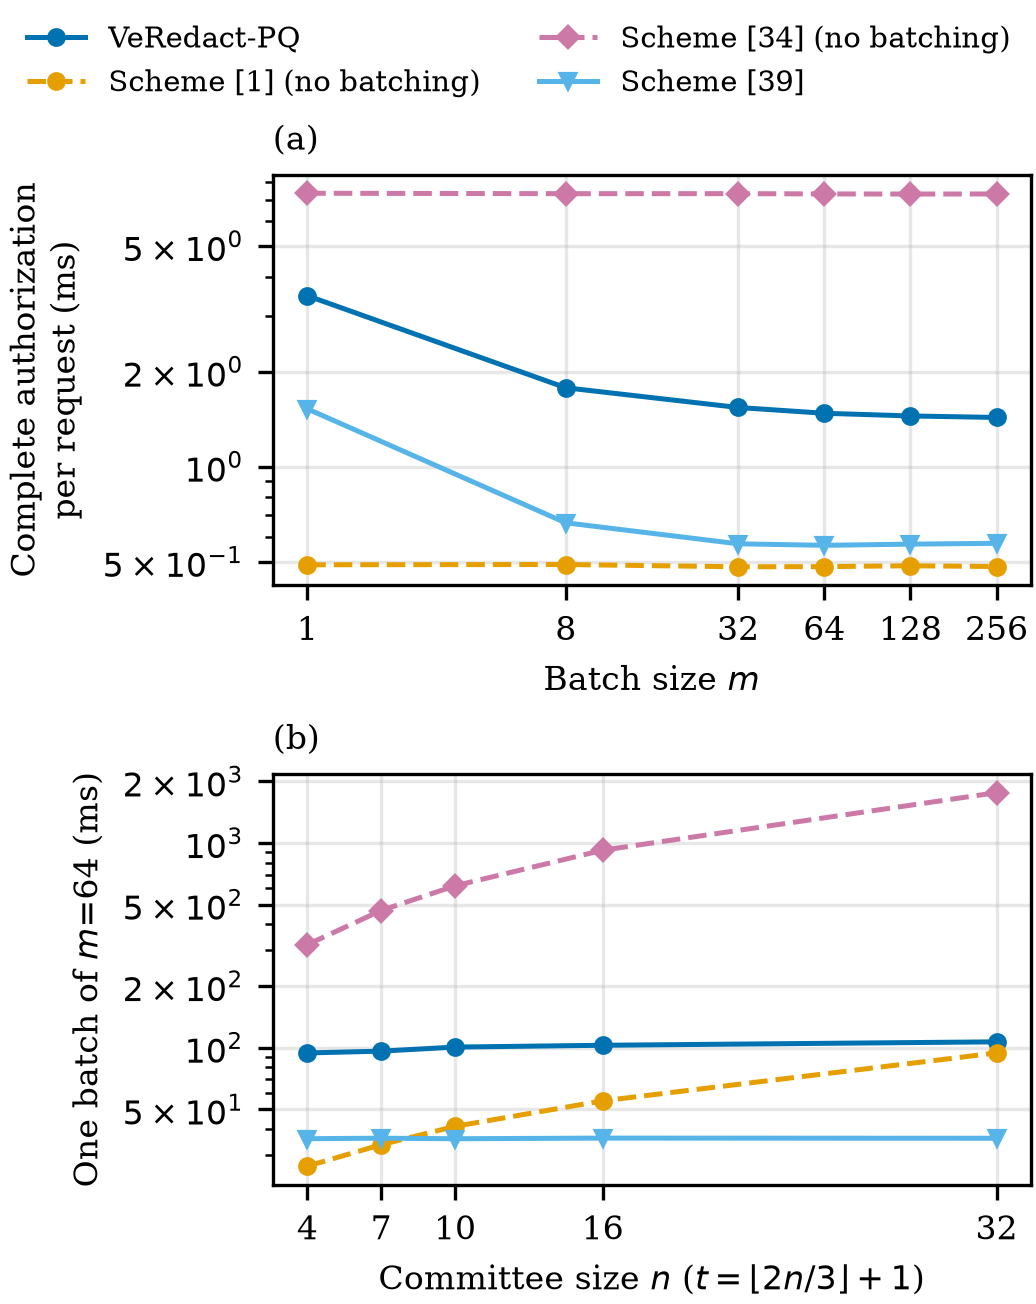
\includegraphics[width=0.8\linewidth]{exp2_authorization_latency.png}
    \caption{Authorization latency \chg{(per-request validation and batch
    authorization)}: (a) per request versus batch size and (b) per batch of
    \chg{$m=64$ requests} versus committee size. \chg{Dashed: schemes
    without a batch protocol.}}
    \label{fig:exp2_auth}
    \end{figure}

    \chg{Fig.~\ref{fig:exp2_auth}(a) shows that the per-request
    authorization latency of VeRedact-PQ decreases from 3.25\,ms at $m=1$
    to 1.70\,ms at $m=8$ and 1.41\,ms at $m=256$, because the $t$ committee
    signatures and their verification are shared by all $m$ requests; the
    remaining 1.3\,ms is the Phase~3 validation of each request, which
    verifies its ML-DSA-65 signature and PQZK proof and signs its validation
    attestation. Schemes~\cite{ref1} and~\cite{ref34} have no batch
    protocol, so their latency stays at 0.47 and 7.2\,ms for every $m$.
    Scheme~\cite{ref1} is faster because its $t$ approving nodes only check
    the accumulator and verify the classical ECDSA signatures of the
    transaction, without a policy or requester proof, whereas
    Scheme~\cite{ref34} is 5.1 times slower than VeRedact-PQ at $m=256$
    because every request requires an attribute-based decryption. The
    post-quantum Scheme~\cite{ref39} decreases from 1.55 to about 0.57\,ms;
    it verifies the requesters' lattice signatures in aggregate but performs
    no policy-compliance or state-freshness check, which accounts for its
    lower latency.}

    \chg{Fig.~\ref{fig:exp2_auth}(b) shows the latency of one batch of
    $m=64$ requests. It increases with committee size for the
    committee-based schemes, from 91 to 102\,ms for VeRedact-PQ, from 26 to
    91\,ms for Scheme~\cite{ref1}, and from 310 to 1{,}726\,ms for
    Scheme~\cite{ref34} as $n$ grows from 4 to 32, while
    Scheme~\cite{ref39}, which has a single verifier and no committee, stays
    at about 36\,ms. For VeRedact-PQ, the committee term is incurred once
    per ABRRR batch and therefore affects each request only through the
    amortized term $t(T_S+T_V)/m$; its latency grows by 11\% from $n=4$ to
    $n=32$, compared with 3.5 and 5.6 times for Schemes~\cite{ref1}
    and~\cite{ref34}. Consequently, larger committees, which strengthen
    distributed control, remain practical under high redaction volumes.}

    % ---------------------------------------------------------------------
    \subsubsection*{\textbf{Experiment 3: Audit Efficiency}}

    This experiment evaluates the service-side efficiency of Phase~6
    auditing, namely query resolution, evidence generation, and response
    size. The number of returned redaction records is varied as
    $n_Q\in\{10,10^2,10^3,10^4,\chg{10^5}\}$, \chg{with records drawn from
    authorization batches of 64 requests}. VeRedact-PQ is compared with
    Scheme~\cite{ref13} and Scheme~\cite{ref1}. Response-generation
    time and response size are measured\chg{, each over 30 queries (5 at $n_Q=10^5$, and 5 for
    Scheme~\cite{ref13} at $n_Q=10^4$)}. The results are shown in
    Fig.~\ref{fig:exp3_audit}.

    \begin{figure}[t]
    \centering
    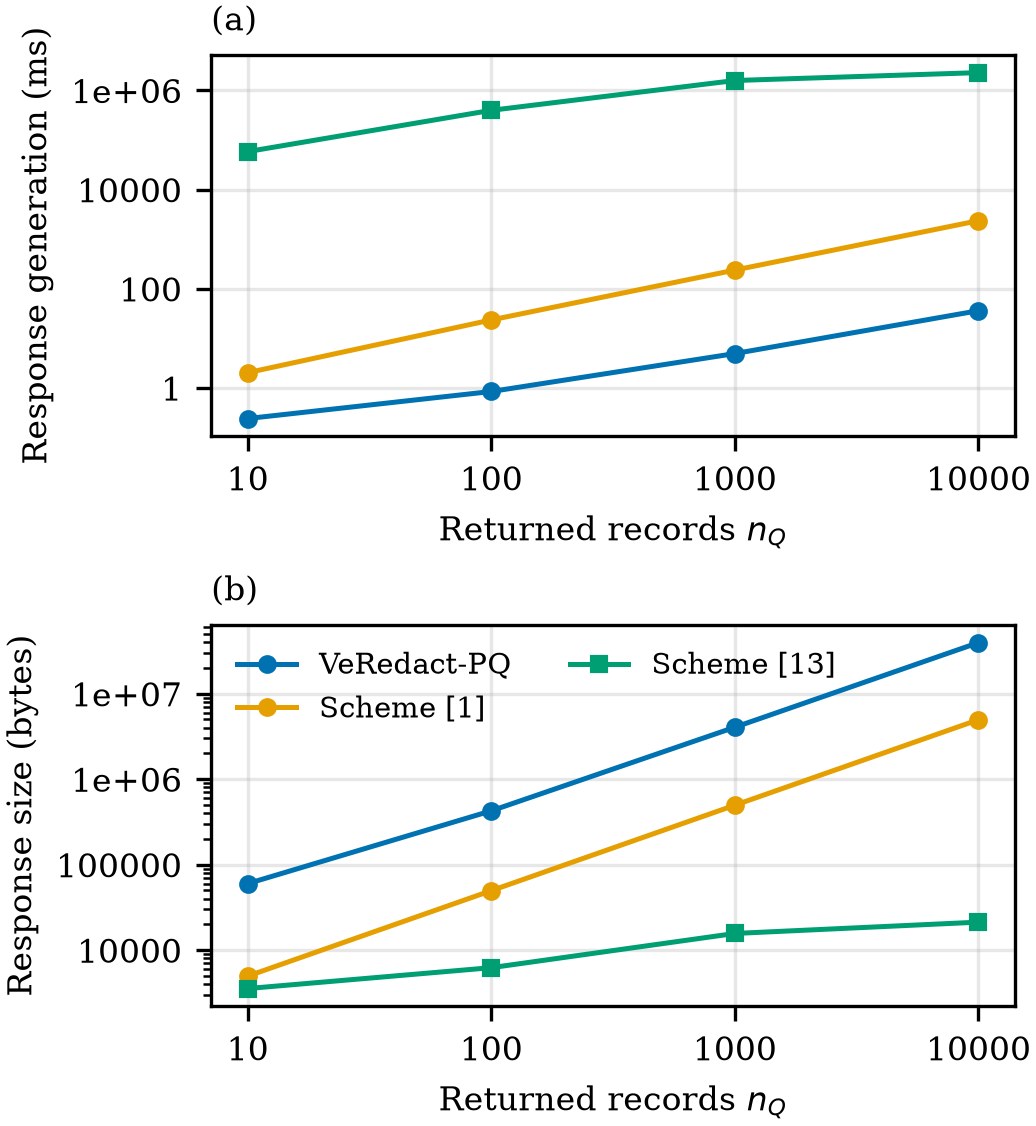
\includegraphics[width=0.8\linewidth]{exp3_audit_efficiency.png}
    \caption{Audit efficiency: (a) response-generation time
    and (b) audit-response size versus the number of returned records.}
    \label{fig:exp3_audit}
    \end{figure}

    \chg{Fig.~\ref{fig:exp3_audit}(a) shows that VeRedact-PQ generates audit
    responses fastest, from 0.38\,ms at $n_Q=10$ to 57\,ms at $n_Q=10^4$
    and 443\,ms at $n_Q=10^5$,
    because records are resolved through the sharded RAI and the
    query-scoped multiproof $MP_{Q_j}^A$ shares internal Merkle nodes.
    Ref.~\cite{ref1} requires 3.3\,ms to 27.7\,s, and Ref.~\cite{ref13}
    requires 11\,min to 73\,h, since it builds one RSA-accumulator
    non-membership witness per returned record.}

    \chg{Fig.~\ref{fig:exp3_audit}(b) shows the opposite ordering for
    response size. VeRedact-PQ returns the largest responses, from 61\,KB to
    395\,MB, about 4\,KB per record, dominated by the 3{,}309-byte ML-DSA-65
    validation attestation $\alpha_i$ carried by each record, whereas the
    shared authorization evidence $(R_e^{VR},C_e^B,Auth_e^B)$ is included
    only once per distinct authorization batch. Ref.~\cite{ref1} returns
    5.0\,KB to 49.6\,MB, and Ref.~\cite{ref13}, which aggregates its proof,
    returns 3.5 to 183\,KB. Overall, the results show that sharded RAI
    resolution and query-scoped evidence keep audit-service computation
    low, while post-quantum signatures dominate the communication cost of
    record-level evidence.}

    % ---------------------------------------------------------------------
    \subsubsection*{\textbf{Experiment 4: Verification Time}}

    This experiment evaluates auditor-side verification of returned
    redaction evidence. The number of verified records is varied as in
    Experiment~3 \chg{for the \textbf{Normal Audit}, which verifies the
    response signature and query binding, the RAI multiproof, committee
    approvals, validation attestations, and the state-transition and PQCH
    checks of every record.} VeRedact-PQ is compared with Refs.~\cite{ref13}
    and~\cite{ref1} in their original classical instantiations. To evaluate
    verification granularity, modified, substituted, and stale evidence is
    additionally injected into \chg{1\%, 5\%, and 10\%} of returned records,
    and the fraction of invalid records individually rejected and valid
    records retained is measured. The results are shown in
    Fig.~\ref{fig:exp4_verify}.

    \begin{figure}[t]
    \centering
    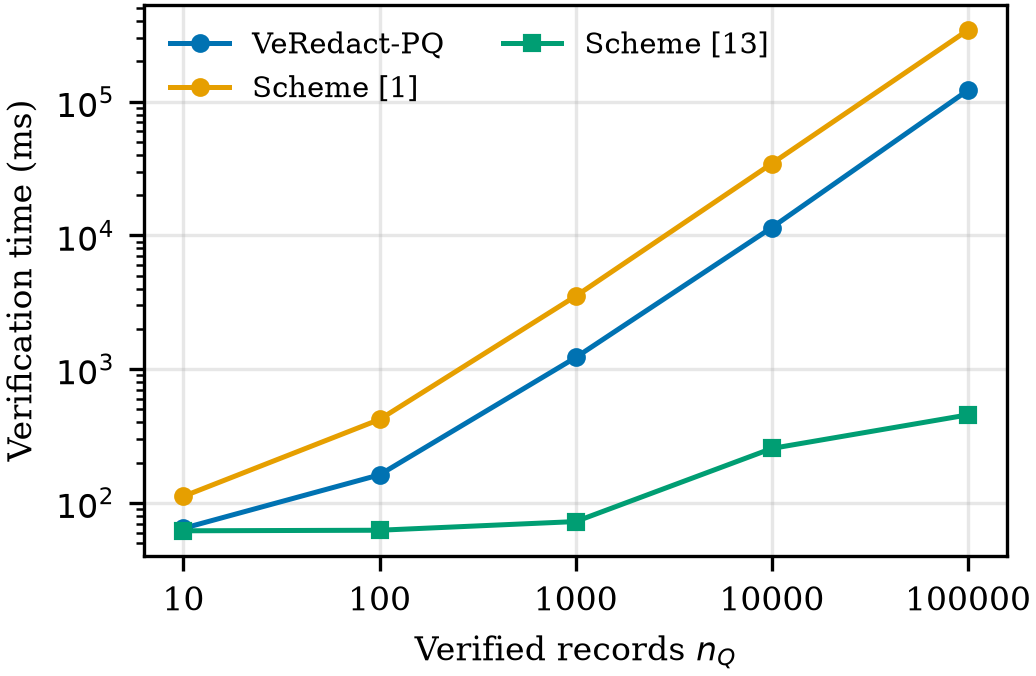
\includegraphics[width=0.8\linewidth]{exp4_verification_time.png}
    \caption{Verification time versus number of verified records for
    \chg{the normal audit}.}
    \label{fig:exp4_verify}
    \end{figure}

    \chg{Fig.~\ref{fig:exp4_verify} shows that normal-audit verification
    time of VeRedact-PQ grows approximately linearly with $n_Q$, from
    64.5\,ms at $n_Q=10$ to 11.5\,s at $n_Q=10^4$ and 121.9\,s at $n_Q=10^5$,
    1.7 to 3.0 times faster than Ref.~\cite{ref1} (111.9\,ms to 343.7\,s).
    Ref.~\cite{ref13} verifies one aggregated proof in 62--455\,ms and is
    therefore faster for large queries. At $n_Q=10^4$, the state-transition
    and PQCH checks, including reading the anchored checkpoints from their
    anchoring blocks, account for 9.9\,s of the 11.5\,s, while committee
    approvals contribute only 59\,ms ($t|\Omega_{Q_j}^B|T_V$); routine audits therefore rely only
    on PQ-signed attestations and hash-based authentication, and complete
    PQZK verification is reserved for challenged or forensic audits.
    Because each returned record carries individual membership and
    execution evidence, VeRedact-PQ and Ref.~\cite{ref1} reject every
    injected modified, substituted, or stale record individually while
    retaining all valid records, as stale evidence fails the version,
    epoch, and checkpoint checks of Phase~6. In contrast, the aggregated
    decision of Ref.~\cite{ref13} rejects the whole response, including all
    valid records, whenever a single record is invalid.}

    % ---------------------------------------------------------------------
    \subsubsection*{\textbf{Experiment 5: Blockchain Gas Consumption}}

    This experiment evaluates the on-chain cost of VeRedact-PQ on the
    permissioned Besu network. Although the gas price is set to zero in the
    permissioned deployment, gas usage provides a deterministic measure of
    on-chain computation and storage. The measured contract operations are
    policy and committee registration (Phase~1), batch-checkpoint anchoring
    $A_b$ (Phase~2), authorization anchoring $H(Auth_e^B)$ (Phase~4), redaction finalization, which atomically commits the
    updated checkpoints $\{A_b'\}$ and SA-RLI state (Phase~5), and RAI
    checkpoint anchoring $CP_e^A$ (Phase~6). \chg{Every scheme finalizes the
    same 1{,}024 requests under Zipf skew $s=0.8$.} The baselines were
    implemented as contracts that store the on-chain redaction state
    prescribed by each scheme\chg{; since none of them defines batching,
    each redaction is its own transaction. The gas per finalized redaction
    is compared across schemes, with VeRedact-PQ both without batching
    ($m=1$) and at its default ABRRR batch size ($m=64$), and the effect of
    the batch size $m\in\{1,8,32,64,128,256\}$ is evaluated for VeRedact-PQ
    alone}. The results are shown in Fig.~\ref{fig:exp5_gas}.

    \begin{figure}[t]
    \centering
    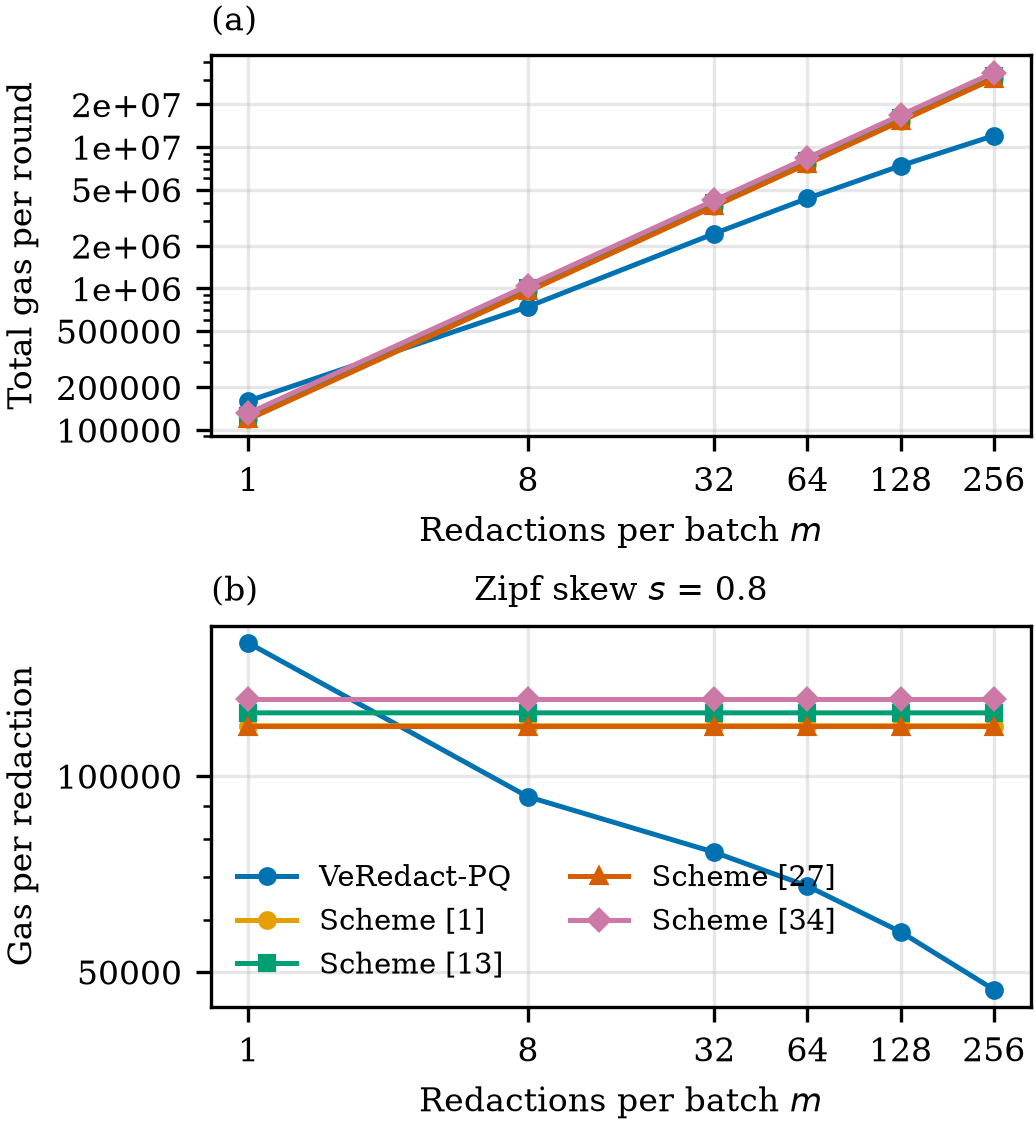
\includegraphics[width=0.8\linewidth]{exp5_gas_consumption.png}
    \caption{Gas consumption: (a) gas per finalized redaction \chg{of each
    scheme} and (b) \chg{gas per redaction of VeRedact-PQ} versus the
    \chg{ABRRR batch size, with the cheapest baseline as reference}.}
    \label{fig:exp5_gas}
    \end{figure}

    \chg{Fig.~\ref{fig:exp5_gas}(a) shows that the baselines consume
    119{,}261 to 153{,}825 gas per redaction, since each redaction updates
    its own on-chain state in one transaction; Scheme~\cite{ref1} is the
    most expensive because each redacted block header also records its
    updated accumulator, which its auditor reads. Without batching, VeRedact-PQ
    consumes 160{,}127 gas per redaction, more than every baseline, because
    each request additionally anchors its authorization $H(Auth_e^B)$. At
    the default batch size of 64, it consumes 81{,}039 gas, 32\% less than
    the cheapest baseline, Scheme~\cite{ref27}. Fig.~\ref{fig:exp5_gas}(b)
    shows that VeRedact-PQ becomes cheaper than Scheme~\cite{ref27} from
    $m=8$ (96{,}294 gas) and reaches 70{,}727 gas at $m=256$, because one
    authorization anchor serves all $m$ requests and redaction finalization
    commits one updated checkpoint per affected transaction batch
    $|\Omega_e|$ rather than per request, while individual redaction records
    are authenticated through the RAI checkpoint.}

    \chg{Table~\ref{tab:gas} further reports the gas consumed by each contract
    operation. Overall, the results show that VeRedact-PQ bounds on-chain
    cost by the number of batch-root transitions and the audit-epoch
    frequency, rather than by the total redaction volume.}

    \begin{table}[t]
    \centering
    \caption{Gas Consumption of VeRedact-PQ Contract Operations}
    \label{tab:gas}
    \scriptsize
    \renewcommand{\arraystretch}{1.08}
    \setlength{\tabcolsep}{4pt}
    \begin{tabular}{lcc}
    \hline
    \textbf{Operation} & \textbf{Frequency} & \textbf{Gas} \\
    \hline
    Policy registration & Per policy version & [TBD] \\
    Committee registration & Per epoch & [TBD] \\
    Batch checkpoint $A_b$ & Per transaction batch & [TBD] \\
    Authorization anchor $H(Auth_e^B)$ & Per ABRRR batch & \chg{44{,}460} \\
    Redaction finalization $\{A_b'\}$ & Per ABRRR batch & \chg{115{,}645 ($|\Omega_e|=1$)} \\
    RAI checkpoint $CP_e^A$ & Per audit epoch & \chg{45{,}811} \\
    \hline
    \end{tabular}
    \end{table}
